\documentclass[12pt]{article}

%%%%%%%%%%%%%%%% Commands for including graphics %%%%%%%%%%%%%%%%%%%
\usepackage{graphicx}
\DeclareGraphicsExtensions{.ps,.eps,.pcx}
%%%%%%%%%%%%%%%%%%%%%%%%%  End of these commands %%%%%%%%%%%%%%%%%
\usepackage{amsmath}
\usepackage{amssymb}
\usepackage{latexsym}
\usepackage{eucal}
\usepackage{color}
\usepackage{multirow}
\usepackage{enumitem}
\setlist{nolistsep}

\usepackage{algorithm}
\usepackage{setspace} % spacing in the algorithm
\usepackage{listings} % code Darstellung

\lstset{ 			  % code style
	backgroundcolor=\color{white},
	keepspaces=true,
	numbers=left,						% where to put the line-numbers
	numberstyle=\tiny\color{black},
	stepnumber=1,						% the step between two line-numbers
	captionpos=b,						% sets the caption-position to bottom
	tabsize=2,  						% sets default tabsize to 2 spaces
	showstringspaces=false,				% underline spaces within strings or not
	columns=flexible,
	%breaklines=true					% enter is breakline
	basicstyle={\small\ttfamily},		% the size of the fonts that are used 
	keywordstyle=\color{blue},
	commentstyle=\color{mygreen},
	stringstyle=\color{red},
	escapeinside={\%*}{*)},
	morekeywords={*,...}
}
\definecolor{mygreen}{rgb}{0,0.6,0}
\textwidth16cm


\textheight23cm

\oddsidemargin0.25cm

\evensidemargin0.25cm

\parindent0cm
\parskip2ex plus0.5ex minus0.5ex
\renewcommand{\baselinestretch}{1.37}
\unitlength1.0cm \headheight0cm \topskip0cm \headsep-1cm

\newcommand{\cov}{\mbox{cov\,}}
\newcommand{\var}{\mbox{var\,}}
\newcommand{\bbo}{\mbox{1}\hspace{-3pt}\mbox{I}}
\renewcommand{\Re}{\mbox{I}\hspace{-2pt}\mbox{R}}

\newtheorem{definition}{Definition}
\newtheorem{theorem}{Theorem}
\newtheorem{corollary}{Corollary}
\newtheorem{proposition}{Proposition}
\newtheorem{lemma}{Lemma}
\newtheorem{remark}{Remark}
\newtheorem{example}{Example}

\newcommand{\keyword}[1]{\textbf{#1}}
\newcommand{\tabhead}[1]{\textbf{#1}}
\newcommand{\code}[1]{\texttt{#1}}
\newcommand{\file}[1]{\texttt{\bfseries#1}}
\newcommand{\option}[1]{\texttt{\itshape#1}}

%---------------------------------------------------------------------------------------
%	BIBLIOGRAPHY SETTINGS
%---------------------------------------------------------------------------------------

\usepackage[backend=bibtex,style=authoryear,natbib=true]{biblatex} % Use the bibtex backend with the authoryear citation style (which resembles APA)

\addbibresource{BIB.bib} % The filename of the bibliography

\usepackage[autostyle=true]{csquotes} % Required to generate language-dependent quotes in the bibliography

%---------------------------------------------------------------------------------------


\begin{document}



\title{Smoothing long memory time series using R}
\author{Yuanhua Feng, Jan Beran and Sebastian Letmathe\\ Faculty of Business Administration and Economics, Paderborn University}
\maketitle
%\doublespacing


%\centerline{\large $^3$Swiss Federal Research Institute WSL}







\begin{abstract}
\noindent 
This paper provides first a brief summary of the SEMIFAR (semiparametric fractional autoregressiove) and ESEMIFAR (exponential SEMIFAR) models. Those models are extended slightly to include the moving average part. Under common distribution condition it is shown that the long memory parameter is not affected by the log-transformation. 
A simple data-driven algorithm is proposed, by which the selected bandwidth and the selected orders of the ARMA model are all consistent. An R package is developed for practical implementation. The application of the proposals are illustrated by different kind of time series. 

  
%

\vspace{.3cm}

\noindent{\it Keywords:} Nonparametric regression with long memory, SEMIFAR, ESEMIFAR, bandwidth selection, model selection, implementation in R, 

%Generalized ESEMIFAR, asymptotic results, bandwidth selection, bootstrap forecasting, long memory in realized volatility

\vspace{.3cm}

\noindent{\it JEL Codes:} C14, C51
\end{abstract}

\newpage

\vspace{.5cm}

%\thispagestyle{empty}

\section{Introduction}
Literature research and model research required.\\
\\ 
In many areas of research data are observed spatially, depending on two separate dimensions in a lattice. 
In recent years one can observe more frequently some sort of apparent memory in the decay of spatial correlations to depend and change over its direction within the spatial process. 
For instance, long-memory in the sense of slowly decaying autocorrelations in (high frequency) financial data across trading time and trading day produces a random field on a lattice in both dimensions simultaneously. \textcite{beran2015modelling} state that daily average trade duration data has often shown long memory
with a clear non zero mode. Therefore a log-normal conditional distribution is suggested.
The simplest approach to model long range dependence in a positive valued
time series is to take the exponential of a linear long memory process such as
FARIMA leading to stochastic volatility models. Due to the long range dependence
there is an unobservable latent process which makes the estimation and interpretation
of the fitted parameters very challenging.\\
\\
The SEMIFAR and ESEMIFAR models introduced by \textcite{beran2002semifar} and \textcite{beran2015modelling} are designed for simultaneous modeling of stochastic trends, deterministic trends and stationary short- and long-memory components in a time series such that the trend generating mechanisms can be distinguished.

\section{Local polynomial regression with long memory}

A well-established model for  analysing financial time series data is the multiplicative error model (MEM) (\cite{engle2002dynamic})  which is given by 
\begin{equation}
\label{MEM}
X_t=s \lambda_t \eta_t,
\end{equation}
where the scale parameter is denoted by $s >0$, $\lambda_t >0$ denotes the conditional mean of $X^*=X_t/s$, and $\eta_t$ are i.i.d. random variables with zero mean and unit variance. Following Feng and Zhou (2015) we can rewrite \eqref{MEM} as a semiparametric MEM given by
\begin{equation}
\label{SMEM}
X_t=s(\tau_t)\lambda_t \eta_t,
\end{equation}   
where $\tau_t=t/n$ denotes the rescaled time and where the scale parameter $s$ in \eqref{MEM} is replaced with a nonparametric scale function denoted by $s(\tau_t)$. 
By taking the logs of \eqref{SMEM} we have
\begin{equation}
\label{SEMIFAR}
Y_t=g(\tau_t) + Z_t,
\end{equation}
where $Y_t=\ln(X_t)$, $g(\tau_t)=\ln[s(\tau_t)]$, $Z_t=\ln(\lambda_t) + \epsilon_t$ and $\epsilon_t=\ln(\eta_t)$. Following \citet{beran2002semifar} we assume that $Z_t$ follows a zero mean FARIMA ($p, d, q$) process 
\begin{equation}
\label{FARIMA}
(1-B)^d\phi(B)Z_t =\psi(B)\epsilon_t,
\end{equation}
where $d \in (0,0.5)$ is the long-memory parameter, $B$ is the backshift operator, $\phi(z)=1-\sum_{i=1}^{p}\phi_iz^i$ and  $\psi(z)=1+\sum_{i=1}^{q}\psi_iz^i$ are AR- and MA-polynomials with all roots outside the unit circle. Equation \eqref{FARIMA} defines a stationary and invertible FARIMA process with $E(\epsilon_t)=0$ and $var(\epsilon_t)=\sigma^2_{\epsilon}$. Model \eqref{SEMIFAR} is equivalent to a SEMIFAR process (\cite{beran2002semifar}) with no integer differencing ($m=0$) and an additional MA-part. We have $X^*_t = \exp(Z_t)$. Subsequently, model \eqref{SMEM} is an extended version of an ESEMIFAR introduced by \citet{beran2015modelling}. However, the authors assumed that $X^*_t$ is log-normally distributed whereas in this paper we relax this assumption and suppose that $X_t^*$ satisfies condition \textbf{A1} of \citet{feng2020fractionally}.
%The long-memory parameter $d$ was introduced by \citet{granger1980introduction} and \citet{hosking1981fractional} and is defined by 
%\begin{equation}
%\label{d}
%(1-B)^{\delta} = \sum_{k=0}^{\infty} b_k(\delta) B^k, 
%\end{equation} 
%where $b_k(\delta) = (-1)^{k}{\delta\choose k}  = (-1)^{k} \frac{\Gamma(\delta+1)}{\Gamma(k+1)\Gamma(\delta-k+1)}$ and $\Gamma(\cdot)$ denotes the Gamma function.

In the following local polynomial estimation of the scale function $g^{(\nu)}$, the $\nu$-th derivative of $g$, is exemplified briefly (see e.g. \cite{beran2002iterative}, \cite{beran2002local}, \cite{beran2002semifar}, and \cite{beran2013limit}). Under the assumption that $g$ is at least ($l+1$)-times differentiable at a point $t_0$, $g(\tau_t)$ can be approximated by a local polynomial of order $l$ for $\tau_t$ in a neighbourhood of $\tau_0$. Following \citet{gasser1979kernel}, the weight function is determined to be a second order kernel with compact support $[-1,1]$ having the polynomial form $K(u)=\sum_{i=0}^{r}a_i u^{2i}$, for $(|u|\leq1)$,where $K(u)=0$ if $|u|>1$ and $a_i$ are such that $\int_{-1}^{1}K(u)du=1$ holds.  Here, $r \in \{0,1,2,3\}$ denotes the kernel used for estimating $g^{(\nu)}$, corresponding to the uniform, epanechnikov, bisquare and triweight kernel.
$\hat{g}^{(\nu)}$ ($\nu\leq l$) can now be obtained by solving the locally weighted least squares problem
\begin{equation}
\label{LP}
Q=\sum_{i=1}^{t}\Bigg[Y_t-\sum_{j=0}^{l}b_j(\tau_i-\tau_0)^j\Bigg]^2 K\Big(\frac{\tau_i-\tau_0}{h}\Big),	
\end{equation}
where $h$ denotes the bandwidth and $K[(\tau_i-\tau_0)/h]$ are the weights ensuring that only observations in the neighbourhood of $\tau_0$ are used. Consider the case where $l-\nu$ is odd. Define $m=l+1$, then we have $m \geq \nu + 2$ and $m-\nu$ is even. A point $\tau$ is said to be in the interior for each $\tau_t\in [h,1-h]$, at the left boundary if $\tau_t\in [0,h)]$ and at the right boundary if $\tau_t\in (1-h,1]$. Following \citet{beran2002local} a common definition for an interior point is $\tau=ch$ with $c=1$ and for a boundary point we have $c \in [0,1)$.   
\citet{beran2002iterative} and \citet{beran2002local}  Asymptotic expressions for the bias, variance and mean integrated squared error (MISE) are presented in Theorem 1 and 2 by \citet{beran2002local}. The asymptotic mean integrated squared error (AMISE) is given by
\begin{equation}
	\label{AMISE}
	\text{AMISE}(h) = h^{2(m-\nu)} \frac{I[g^{(m)}]\beta^2}{m!} + \frac{(nh)^{2d-1}V(1)}{h^{2\nu}},
\end{equation}
where $I[g^{(m)}] = \int_{c_b}^{1-d_b}[g^{m}(\tau)]^2d\tau$ with $0 \leq c_b < d_b \leq 1$ in order to reduce the so-called boundary effect. Moreover, $\beta = \int_{-1}^{1}u^mK(u)du$ and for $d > 0 $ we have $V(1)=2c_f \Gamma(1-2d)\sin (\pi d) \int_{-1}^{1} \int_{-1}^{1} K(x)K(y)|x-y|^{2d-1}dxdy$. For $d = 0$, $V$ reduces to $V(1)=2\pi c_f \int_{-1}^{1}K^2(x)dx$. $c_f$ stands for the spectral density of the ARMA part of \eqref{FARIMA} at frequency zero and is given by 
\begin{equation}
	c_f = f(0) = \frac{\sigma^2_\epsilon}{2\pi} \frac{(1 + \psi_1+\dots+\psi_q)^2}{(1-\phi_1-\dots-\phi_p)^2}.
\end{equation}
 The asymptotically optimal bandwidth, denoted by $h_A$, that minimizes the AMISE is given by
\begin{equation}
	\label{ha1}
h_A=Cn^{(2d-1)/(2m+1-2d)},
\end{equation}
with 
\begin{equation}
\label{ha2}
C=\Bigg(\frac{[m!]^2}{2(m-\nu)} \frac{(2\nu+1-2d)}{\beta^2}\frac{(d_b - c_b)V(1)}{I[g^{(m)}]}\Bigg)^{1/(2m+1-2d)}.
\end{equation}
Based on these results \citet{beran2002iterative} proposed two iterative plug-in algorithms for automatic bandwidth selection, namely Algorithm \textbf{A} and \textbf{B}. In this paper we only consider a strongly adapted version of Algorithm \textbf{B} which is presented in the following.


 
%\subsection{The E-SEMIFARIMA}
%In the context of modelling long-range dependence and deterministic trends in trade duration series \citet{beran2015modelling} introduced the ESEMIFAR model defined by equation 
%
%A theorem about the memory property of the ESEMIFAR (direct after that model) 
%\begin{theorem}
%Assume that $X_t$ follows an ESEMIFAR model defined above with $d>0$ and a linear FARIMA error process $\xi_t$ in the log-data, then $Z_t=X_t/v(\tau_t)$ is a stationary long memory process with the same memory parameter $d$.   
%\end{theorem}
%This result shows that the level of long memory of the stationary part of the process under consideration is not affected by the log- or exponential transformations. In the case when $\xi_t$ is normal, those results are e.g. obtained in Dittmann and Granger (2002) and Beran et al. (2015). Theorem 2 extends those results to a common innovation distribution in the log-data. The proof of Theorem 2 is given in the appendix, where we will show that the process $Z_t$ is a special case of the general framework defined in Surgailis and Viano (2002). Hence, their results apply to $Z_t$. Note however that the above result does not hold for $d=0$. Detailed discussion on corresponding properties in case with $d=0$ is beyond the aim of the current paper.  

\section{Data-driven estimation}
In order to obtain a selected bandwidth the unknown constants $I[g^{(m)}]$, $d$ and $V$ in \eqref{ha1} have to be replaced with consistent estimators. Please note, that the estimation of $V$ relates to that of $cf$. $I[g^{(m)}]$ is estimated by means of local polynomial regression and numerical integration. The remaining two quantities $d$ and $V$ can be obtained via maximum likelihood. Inserting those estimates into \eqref{ha1} yields a plug-in estimator for the bandwidth, which minimises the MISE.

\subsection{The IPI-algorithm for estimating $g$}

We introduce an IPI-procedure for SEMIFARIMA models by translating and adapting the main features of the IPI for SEMIFAR models introduced by \citet{beran2002iterative} from the programming language \texttt{S} to \texttt{R}. The algorithm processes as follows:

\begin{itemize}
	\item[\textbf{i)}] In the first iteration start with an initial bandwidth $h_0$ set beforehand and select $p$ and $q$ denoting the AR- and MA-order, respectively. 

	\item [\textbf{ii)}] Estimate $g$ from $Y_t$ employing $h_{j-1}$ and calculate the residuals $\tilde{Z}_t = Y_t - \hat{g}(\tau_t)$. Estimate $d$ and $V$ by fitting a FARIMA (with predefined AR- and MA-order in Step i) to  $\hat{Z}_t$.
			
	\item [\textbf{iii)}] Set $h_{d,j}=(h_{j-1})^\alpha$, where $\alpha$ denotes an 
		inflation factor. Estimate $I[g^{(m)}]$ via a local polynomial of order $l^* = l + 2$ and with $h_d,j$. Now, we obtain $h_{j-1}$ by 
		\begin{equation}
			h_j=\Bigg(\frac{[m!]^2}{2m} \frac{(1-2\hat{d})}{\beta^2}\frac{(d_b - c_b)\hat{V}(1)}{I[\hat{g}^{(m)}]}\Bigg)^{1/(2m+1-2\hat{d})}\cdot n^{(2\hat{d}-1)/(2m+1-2\hat{d})}.
		\end{equation}
	
	\item [\textbf{iv)}] Repeat steps ii) and iii) until convergence or a given number of iterations has been reached and set $\hat{h}_{opt} = h_j$.	
\end{itemize}
We propose to set the initial bandwidths to $h_0 = 0.1$ for $l = 1$ and $h_0 = 0.2$ for $l = 3$. Moreover, for $p = 3$ it is recommended to employ $c_b = 1 - d_b$ such that only 90\% of all observations are used for estimating an interior point in order to reduce the boundary effect. For $l = 1$ all observations are used and hence $c_b = 1 - d_b = 0$. The bandwidth $h_{d.j}$ used for estimating $g^{(m)}$ is enlarged by means of an exponential inflation factor denoted by $\alpha$. We have $\alpha = \alpha_{\text{opt}} = (2m + 1 - 2d) / (2m + 3 - 2d)$, $\alpha = \alpha_{\text{nai}} = (2m + 1 - 2d) / (2m + 5 - 2d)$ and $\alpha = \alpha_{var} = \frac{1}{2}$. Using $\alpha_{\text{opt}}$ results in bandwidth $h_{d,j}$ that minimizes the MSE of $\hat{I}[g^{(m)}]$ and consequently the rate of convergence of $\hat{h}_j$ is optimal. Whereas for $\alpha_{\text{nai}}$ the optimal rate of convergence is achieved for $\hat{m}^{(m)}$ and $\alpha_{\text{var}}$ ensures a stable selection of the bandwidth. Moreover, we have $\alpha_{\text{var}} > \alpha_{\text{nai}} > \alpha_{\text{opt}}$ and $\alpha_{\text{nai}} \rightarrow \alpha_{\text{var}}$ as $d \rightarrow 0.5$. The choice of $\alpha$ depends on the underlying data, which is to be analysed. For a more detailed insight on inflation methods we refer the reader to \citet{beran2002iterative} among others.   

%Please note that the results presented in \citet{beran1999semifar}, \citet{beran2001volatility}, \citet{beran2002iterative}, \citet{beran2002local}, \citet{beran2002semifar} and \citet{beran2016long} remain valid for the IPI for SEMIFARIMA models.    

\subsection{Data-driven estimation of g\textquotesingle{} and g\textquotesingle \textquotesingle}
The IPI for SEMIFARIMA models can also be applied to bandwidth selection for estimating $g^{(\nu)}$ with $\nu > 0$. In this paper, only the cases for $\nu = 1$ and $\nu = 2$ are discussed. The proposed IPI is now employed as a data-driven pilot method to obtain estimates for $d$, $c_f$ and $h_{\nu, 0}$ with order $l_d$, say. Estimation of $g^{(\nu)}$ is then carried out with $l = \nu + 1$ and $m = \nu + 2$. As previously, $g^{(m)})$, which is required for calculating $I[g^{(m)}]$ is estimated with order $l^* = l + 2$. The following two-stage procedure is proposed.
\begin{itemize}
	\item[\textbf{i)}] In the first stage $\hat{d}$, $\hat{c}_f$, and $\hat{h}_{\text{opt}}$ are obtained by means of the main IPI-algorithm for estimating $g$ with order $l_d = 1$ or $l_d = 3$.
	
	\item[\textbf{ii)}] Set $h_{\nu,0} = \hat{h}_{\text{opt}}$. Carry out an IPI-procedure as proposed above with fixed $\hat{c}_f$ and $\hat{d}$ in order to select a bandwidth for estimating $g^{(\nu)}$. Please note that \eqref{ha1} should be used. 
\end{itemize}
Explicit formulas of the equivalent kernels for estimating $g^{(\nu)}$ at an interior point $\tau_t$ can be found in \citet{muller1988longitudinal}. The corresponding inflation factors are defined as previously and are determined by $m$ and $d$.

\section{Implementation in R}
Based on the algorithms introduced in the previous section a R-package is currently developed, which is an extension of the already published \textit{smoots} package. Hence, this package will be coined \textit{smootslm}. The main functions are called \textit{tsmoothlm} and \textit{dsmoothlm} for estimating the trend and its derivatives, respectively, under presence of long-memory errors. Local polynomial estimation of  $g^{(\nu)}$ and kernel smoothing of $g$ are carried out by means of the functions \textit{gsmooth} and \textit{knsmooth}, which are implemented in the \textit{smoots} package (see Feng et al., 2020).

In the following the function \textit{tsmoothlm} is explained in more detail. The first argument $y$ denotes the input time series. The second and third argument (\textit{pmin} and \textit{pmax}) are the minimum and maximum AR-order of the stochastic part $Z_t$ in \eqref{SEMIFAR}, respectively. Accordingly, the fourth and fifth argument (\textit{qmin} and \textit{qmax}) stand for the the minimum and maximum MA-order of $Z_t$. All four arguments can take the value 0, 1, 2, 3, 4 or 5 while $p_{\text{min}} \leq  p_{\text{max}}$ and $q_{\text{min}} \leq  q_{\text{max}}$. The optimal order is determined via BIC. The default setting is $p_{\text{min}} = q_{\text{min}} = p_{\text{max}} = q_{\text{max}} = 0$. The order of the polynomial for trend estimation is set via the argument $p$ and the user can choose between 1 and 3, where $p = 1$ is the predefined option. The argument \textit{mu} controls for the smoothness of the weight function. We have $\mu \in \{0,1,2,3\}$, with $\mu = 1$ for the Epanechnikov kernel as default. Furthermore, the inflation factor $\alpha$ can be selected by the argument \textit{InfR} with three different options, i.e. \textit{"Opt"}, \textit{"Nai"} and \textit{"Var"}, which corresponds to $\alpha_{\text{opt}} = (2m + 1 - 2d) / (2m + 3 - 2d)$, $\alpha_{\text{nai}} = (2m + 1 - 2d) / (2m + 5 - 2d)$ and $\alpha_{var} = \frac{1}{2}$, respectively.
Moreover, the starting bandwidth $h_0$ can be set beforehand by the argument \textit{bStart} with default $h_0 = 0.1$ for $p =1$ and $h_0 = 0.2$ for $p = 3$. However, the choice of \textit{bStart} should not affect the finally selected bandwidth if the IPI converges. Argument \textit{bb} controls for boundary bandwidth. The default is $bb = 1$ meaning that the k-nearest neighbour method is applied, which results in a total bandwidth of $2\hat{h}$ at each observation point $\tau_t$. For $\textit{bb} = 0$ however, the total bandwidth is shortened at boundary points. By the argument \textit{cb}, which is set to $\textit{cb} = 0.05$ per default, the percentage of observations omitted for calculating $I[g^{(m)}] = \int_{c_b}^{1-d_b}[g^{m}(\tau)]^2d\tau$ in \eqref{ha1} can be controlled. Additionally, the smoothing method with $\hat{h}_{\text{opt}}$ can be selected via the argument \textit{method}. The user may choose between local polynomial regression ("\textit{lpr}") and kernel regression ("\textit{kr}"). However, originally kernel regression has been only incorporated in the \textit{smoots} package as a comparison to local polynomial regression.

For estimating $g^{(\nu)}$ the function \textit{dsmoothlm} is applied. Please recall that here \textit{tsmoothlm} is employed as a pilot method with minimum and maximum AR- and MA-order \textit{pmin.p}, \textit{pmax.p}, \textit{qmin.p} as well as \textit{qmax.p}, a local polynomial estimator of order \textit{pp}, the inflation rate \textit{InfR.p}, the kernel \textit{mu.p} and a starting bandwidth \textit{bStart.p} in order to obtain reasonable estimates for $\hat{d}$, $\hat{c_f}$ and $\hat{h}_{\nu,0}$ (see section 3.2). The options and default settings for these arguments are the same as for \textit{tsmoothlm}. In addition to that, the order of the derivative to be estimated is set via the argument \textit{nu} and can take the value 1 or 2 for the first and second derivative, respectively. Moreover, the argument \textit{mu} controls the kernel used for bandwidth selection after the pilot stage. Please note that the S3 methods (\textit{print} and \textit{plot}) implemented in the \textit{smoots} package can be employed to the estimation results of the functions above. The output objects of \textit{tsmoothlm} and \textit{dsmoothlm} are basically lists containing input parameters and estimation results. Furhter detailed information on the functions are to be published in the users guideline of the \textit{smootslm} package.       

%The implementation of the SEMIFAR model in \code{R} is called via the \code{semifar.lpf} function. 
%The script covers the kernel estimation of a nonparametric trend allowing for different error structures and maximum likelihood estimation of the parametric part of the model. The \code{R} function is designed for a fast and uncomplicated application of SEMIFAR and assumes some not necessarily fixed values a priori to be constant. For instance, the level of confidence used for \( \eta \) is by default set to \(0.05\) and is among other constants not included as input. Nevertheless the script can be made more flexible very easily by using more parameters in the function call. 
%%It serves as parent for all other
%%function calls and as interface for the whole script. Therefore one has to control the circumstances accounting best for the investigated time series by the input given to \code{semifar.lpf}.
%Besides the series there are currently seven variables to be set before the model is fitted.
%The minimal autoregressive order \(p\), the maximal order \(p\), the range of the MSE of the trend estimate, the degree of the polynomial approximating the nonparametric trend and its derivatives, the used kernel, the inflation factor inflating the previously estimated bandwidth and whether boundary protection is included or not. \\
%\\
%Fitting a SEMIFAR process with the IPI algorithm required the purchase of the TIBCO Spotfire software \code{SPLUS} and the additional \code{FinMetrics} package based on the \code{S} language. To this date, the \code{semifar.lpf} function has successfully been implemented into the language R.
%Major differences in computation are found in 
%\begin{enumerate}
%	\item[1.] the derivation of the ML parameter estimates for a fractionally-differenced ARIMA model, especially for the fractional filter \( \delta \)
%	\item[2.] how the residuals of fractionally filtered data for an ARIMA model are obtained 
%	\item[3.] the calculation of the spectral density and its update
%	\item[4.] a newly introduced inflation factor for bandwidth convergence  
%\end{enumerate}
%Concerning the first point, the difficulty in calculating \( \delta \) comes with introducing antipersistent trend behavior allowing \( \delta < 0 \) and extending the interval of possible values for the \code{drange} to \((-0.5,0.5)\). 
%The main part of producing \( \delta \) is given in \eqref{eq:fractional difference 1} and implements the gamma function and the backshift operator in an infinte binomial sum over \(k\) subtracted from one such that  \(1 - \delta B - \frac{1}{2}\delta(1-\delta) B^{2} - \frac{1}{6} \delta(1-\delta)(2-\delta)^{2} B^{3} - \ldots\) which gives \(  1 - \sum_{k=1}^{\infty} c_k(\delta) B^{k} \). 
%For negative \( \delta \) the signs reverse and the expression is \(< 0\).
%However, the values in the interval \code{drange} in \code{fracdiff\{fracdiff\}} (over which the likelihood function is maximized as a function of \( \delta \)) cannot exceed \(0.5\) since the binomial approaches \(0\) for \( \delta = |\{-0.5,0.5\}| \) and the series would be non stationary.
%Still, having \(\delta\) set to \((-0.5,0.5)\) is crucial for the identification of the trend mechanism of the SEMIFAR process, as the spectral density \(f_{X}(\lambda) \sim \lbrace0,c,\infty\rbrace\) for \(\delta\) in \(\lbrace(-0.5,0),0,(0,0.5)\rbrace\) in order to obtain the autocovariance behavior at the \(0\)th frequency \(f_X(0) = \frac{1}{2 \pi} \sum_{k=-\infty}^{\infty}\gamma_{X}(k) = \lbrace0,c,\infty\rbrace\) expressing the memory structure of the process.
%Therefore a decision criteria for setting \code{drange} to \((0,0.5)\) or to \((-0.5,0)\) is introduced. 
%If either of the specified intervals for \code{drange} does not allow the computation of a correlation matrix of the parameter estimates, the alternative \code{drange} is chosen. 
%In this way, the underlying temporal dependence structure of the data has to correlate positively with the fractional filter. Otherwise there must not be a correlation matrix. 
%\begin{lstlisting}[language=Python]
%> m1=fracdiff(data,drange = c(0,0.5))
%> m2=fracdiff(data,drange = c(-0.5,0))
%> if(isTRUE(all.equal(m1$correlation.dpq,NULL))){result<-m2} 
%> if(isTRUE(all.equal(m2$correlation.dpq,NULL))){result<-m1} 
%\end{lstlisting}  
%By implementing two different persistence situations, \code{fracdiff} objects and a decision criterion, the fractional parameter 
%is successfully estimated and equivalent to \code{arima.fracdiff} output in \code{S}. \\
%\\
%The second change accounts for a different filtering technique used to obtain the residuals and variance of the fractionally filtered ARIMA process. 
%The residuals account for the difference between an estimated and observed value.
%%Therefore, first the fractional and then the ARMA adjustment is applied to the (differenced) series.
%While in \code{S} a dynamic linear Kalman filter is employed to calculate the residuals, a much simpler autoregressive moving average filter is used in \code{R}.
%%
%The Kalman filter predicts the future state of the series %in \(t+1\) 
%based on the current state vector %in \(t\) 
%times the change in time and gives the expected subsequent state.  
%The previous predicted state is corrected using a current sensory measurement %in \(t\) 
%as innovation of the state estimate. 
%However, the innovation is weighted relative to the prediction each time step. Its weight decreases if the current measurement matches the last predicted state and increases otherwise. 
%%The Kalman-Gain is set as the uncertainty about the state times the measurement divided by the covariance and uncertainty of the measurement. 
%%
%%Then the series is filtered for its ARMA component since the Kalman filter eliminates the autoregressive and moving average behavior by
%%Hence, theeach time step and determines 
%Hence, the ratio of uncertainty in measurement and prediction set by the estimated ARMA parameters, filters for short memory and produces the residuals.
%An approach more straightforward is the successive application of standard recursive and convolution filtering methods for four different  model order- and parameter estimates as filter input for the new \code{arma.filt} function.
%In this way all possible ARMA(p,q) contributions to short memory are addressed. 
%Convolution filtering % conceptually 
%%describes the folding or product of two functions 
%uses the product of different functions as weighted average and thus creates an individually weighted mean for each observation (therefore moving average) in line with
%\begin{equation}
%\label{eq:ConvolutionFilter}
%I(x,y) = \sum_{s=-i}^{i} \sum_{t=-j}^{j} w(s,t) (x-s,y-t).
%\end{equation}
%Hence there are at least \(max\left\lbrace p,q \right\rbrace \) \code{NA}s for each filter value. 
%The recursive filtering method describes the re-use of its output as input which is also done within the Kalman filter. The filtered values will exceed their input values for positive \(w_j\) and will be lower for \(w_j <0\). The recursive filter method is given by
%\begin{equation}
%\label{eq:RecursiveFilter}
%y_t = \sum_{j=0}^{J} y_{t-j} w_j,
%\end{equation}
%where \( J \) is the set of filter criteria. Combining both filter mechanics ensures the consistent elimination of the short memory ARMA component moving the input series. Due to the recursive nature of the AR filter, the MA filter obviously has to be applied before the recursive filter. 
%It is important to use the (fractionally) pre-filtered data since otherwise the filter will rule out movement which does not reflect short memory exclusively. \\
%\\
%The third difference comes with the calculation of the spectral density update. 
%\code{S} and \code{R} produce identical output, apart from the density spectrum which is no longer estimated in decibels such that the transformation \code{f=10**f\$spec/10} is redundant and only \code{f=f\$spec} remains.
%Moreover the frequency of the input \code{xfreq} can be fixed to one since we are considering an univariate time series.\\
%\\
%The fourth change also concerns the update cycle by allowing different factors \( \alpha \) used for inflating the previous bandwidth estimate in \eqref{eq:Bandwidth}. The inflation method significantly changes the rate of convergence \parencite{beran2002iterative}.
%The optimal rate of convergence \(h_M\) expresses a trade-off between a bias and variance ratio producing an overall fit of the trend which is sufficiently stable while being sufficiently smooth. The \code{semifar.lpf} function offers the choice for three different inflation factors called \code{var}, \code{naive} and \code{opt}.
%If \( \alpha \) is chosen as  \(\alpha_{opt} = (5-2\delta)/(7-2\delta)\) and \(\delta\) is for simplicity assumed to be zero, than we have respectively
%\begin{equation}
%\label{eq:IFopt}
%\begin{split}
%\hat{h} & = h_M\left\lbrace 1 + O(n^{2(2\delta-1)/(7-2\delta)}) + O_{p}(n^{2(2\delta-1)/(7-2\delta)}) + O_p(n^{(-1/2)}) \right\rbrace \\
%& = h_M\left\lbrace 1 + O(n^{-2/7}) + O_{p}(n^{-2/7}) + O_{p}(n^{-1/2}) \right\rbrace
%\end{split}
%\end{equation}
%where the first term gives the order of the bias under this particular inflation factor and the second term corresponds to the order of the variance. The third term is asymptotically negligible and for all choices of \( \alpha \) the same.
%The overall rate of convergence under this inflation factor is \(O(n^{-2/5})\).
%The lower bound of the variance is given if \( O_p(n^{-1/2}) \) since \(\delta\) is in \((-0.5,0.5)\) and the rearranged exponent contains \(\delta-1/2\) which is zero if the maximal value of \(\delta\) is inserted.  
%%The index \code{2} in \code{IFM[2]} selects the \code{naive} inflation factor with \(\alpha_{0} = (5-2\delta)/(9-2\delta)\) resulting in 
%%\begin{equation}
%%\label{eq:IFnaive}
%%\begin{split}
%%\hat{h} & = h_M\left\lbrace 1 + O(n^{2(2\delta-1)/(9-2\delta)}) + O_{p}(n^{4(2\delta-1)/(9-2\delta)}) + O_p(n^{(-1/2)}) \right\rbrace \\
%%& = h_M\left\lbrace 1 + O(n^{-2/9}) + O_{p}(n^{-4/9}) + O_{p}(n^{-1/2}) \right\rbrace
%%\end{split}
%%\end{equation}
%%and analogous the index \code{3} selects the \code{opt} inflation factor with \(\alpha_{opt} = (5-2\delta)/(7-2\delta)\) which gives
%%The overall rate of convergence under this inflation factor \code{opt}  with \(\delta = 0\) is \(O(n^{-2/5})\). 
%If the model includes persistent behavior and \(\delta\) is non zero the rate of convergence is slower for \(\delta > 0\) and respectively 
%for \(\delta < 0\) the rate of convergence is faster. 
%%Recall the long memory case featuring a slowly decaying autocorrelation function supporting the deceleration of the convergence for a positive fractional differencing parameter.  
%Depending on \( \alpha \), either the variance term or the bias is of a smaller order and changes smoothing or stabilizes the trend function more.
%In general the best overall rate of convergence is achieved by applying an inflation factor \(\alpha\) that minimizes the bias and variance of the SEMIFAR model.

%The technical implementation in \code{R} is provided in the standard \code{filter::stats} function with \code{method="convolution"} which is also the default. 
%Considering for instance a series \code{x=0:5} from zero to five in a situation with three moving average filter coefficients \code{w[j]} equal to \code{1,2,3} with \code{j=1,2,3} the filter will produce 
%\begin{lstlisting}[language=Python]
%> filter(x,c(1,2,3), method = "conv")
%[1] NA  4 10 16 22 NA
%\end{lstlisting}
%since, for instance \code{x[2]=1} yields a filtered value of 
%\code{x[i-1]*w[3]+x[i]*w[2]+x[i+1]*w[1]}
%which equals \code{4}. 
%The \code{NA}s in are printed due to the missing values of \code{x} at the beginning and the end of the series if \code{i} is at the borders.
%the residuals \code{rBIC}

%https://www.bzarg.com/p/how-a-kalman-filter-works-in-pictures/#mathybits



\section{Application to different kinds of time series}
In this and the following sections the SEMIFARIMA and ESEMIFARIMA are applied to four real data examples: \textit{tempNH} (mean monthly temperature changes), \textit{gdpGER} (GER GDP), \textit{dax} (German stock index) and \textit{vix} (CBOES volatility index). The \textit{tempNH} data set has already been subject to an application example in \citet{feng2007asymptotic}, where the author employed the original version of the IPI for SEMIFAR models. The remaining three data sets have been already used by Feng et al. (forthcoming) and are implemented in the \textit{smoots} package, which was recently published on the \textit{CRAN} network. 

\subsection{Application to environmental data}
The SEMIFARIMA model defined by \eqref{SEMIFAR} and \eqref{FARIMA} is applied to the time series of mean monthly Northern Hemisphere temperature changes (NHTM) from 1880 to 2018. The data is available at the website of the National Aeronautics and Space Administration (NASA). Bandwidth selection is carried out by means of the IPI for SEMIFARIMA models introduced in section 3. For model- and bandwidth selection the \textit{tsmoothlm} function is applied, with $\textit{p} = 1$, $\textit{pmin} = \textit{qmin} = 0$, $\textit{pmax} = \textit{qmax} = 3$ and $\textit{InfR} = \textit{"Opt"}$. The remaining arguments are set on their default. 

In Figure 1a) the fitted trend together with the observations is illustrated. The optimal bandwidth is $\hat{h}_{\text{opt}} = 0.165$ and a FARIMA ($0, \hat{d}, 0$) has been selected following the BIC with $\hat{d} = 0.405$ implying strong long-range dependence in the temperature data. Apparently, the SEMIFARIMA captures the trend quite well. A clear upward trend can be observed approximately after 1970, which could be interpreted as an indicator for global warming. The trend-adjusted residuals are shown in Figure 1b) and first and second derivative are depicted in Figures 1c) and 1d), respectively. Please note that for the estimation of derivatives the dependence structure has been estimated by pilot smoothing with order $\textit{pp} = 3$. The derivatives match the features of the trend shown in Figure 1a) and provide further information about global temperature changes. For instance the slope of the first derivative indicates how strong the trend is increasing or decreasing. The intersections of the second derivative with the x-axis indicate a shift in the slope of $\hat{g}$. 
 
\begin{figure}[h]
		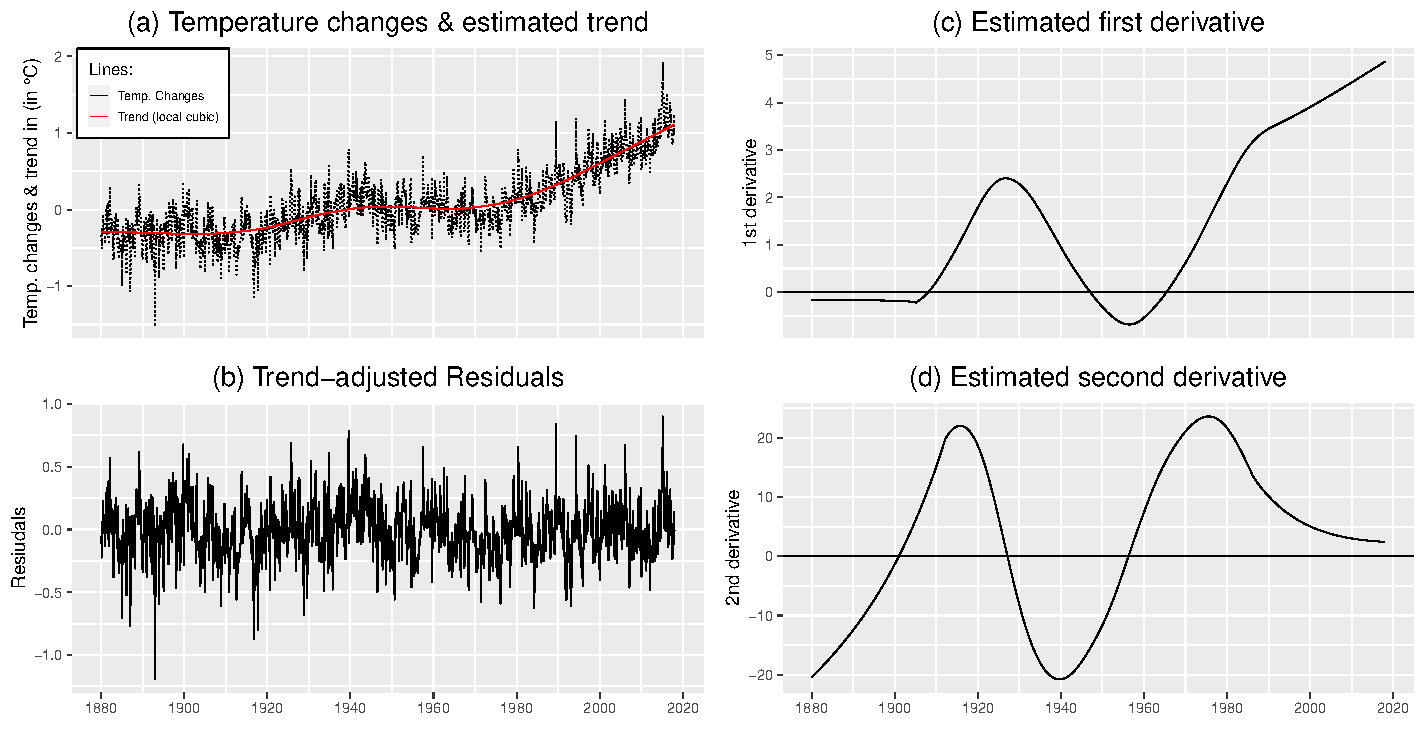
\includegraphics[trim = {0cm 0mm 0mm 0mm}, width = \textwidth]{Abb/NHtemp.pdf}
		\caption{Estimated trend, residuals and the trend`s derivatives for the NHTM series}
\end{figure}



\subsection{Application to GDP data}
A model which is commonly used in the field of macroeconomic research is the well-known log-linear growth model. Feng et al. (2020) have achieved a semiparametric local-linear extensions of this model by applying a Semi-ARMA to log-transformed GDP series. We follow this approach and additionally incorporate long memory by assuming that the log-transformed annually GER-GDP series from 1850 to 2016 follows a SEMI-FARIMA defined by \eqref{SEMIFAR} and \eqref{FARIMA}. For this purpose the \textit{tsmoothlm} function is employed, with $\textit{p} = 1$, $\textit{pmin} = \textit{qmin} = 0$, $\textit{pmax} = \textit{qmax} = 3$ and $\textit{InfR} = \textit{"Opt"}$. The remaining arguments are set on their default. We obtained an optimal bandwidth of 0.161 and a FARIMA ($2,\hat{d},2$) model given by

\begin{equation}
	Z_t = -0.134 Z_{t-1} + 0.542 Z_{t-2} + \frac{(1.363 \epsilon_{t-1} + 0.275 \epsilon_{t-2} + \epsilon_t)}{(1-B)^{0.191}}.
\end{equation}
As a benchmark a kernel regression is carried out using the same bandwidth. Estimated trends together with log-gdp series are shown in Figure 2(a). At the interior both estimators are approximately equal. However, we can see that the kernel estimator clearly shows poor estimation quality at the boundaries which indicates that the local-linear estimator is to be preferred. The trend-adjusted residuals obtained by the local-linear approach are depicted in Figure 2(b). Moreover, the corresponding derivatives are illustrated in Figures 2(c) and 2(d), which reveal further information on the course of the German economy.
 
\begin{figure}[h!]
	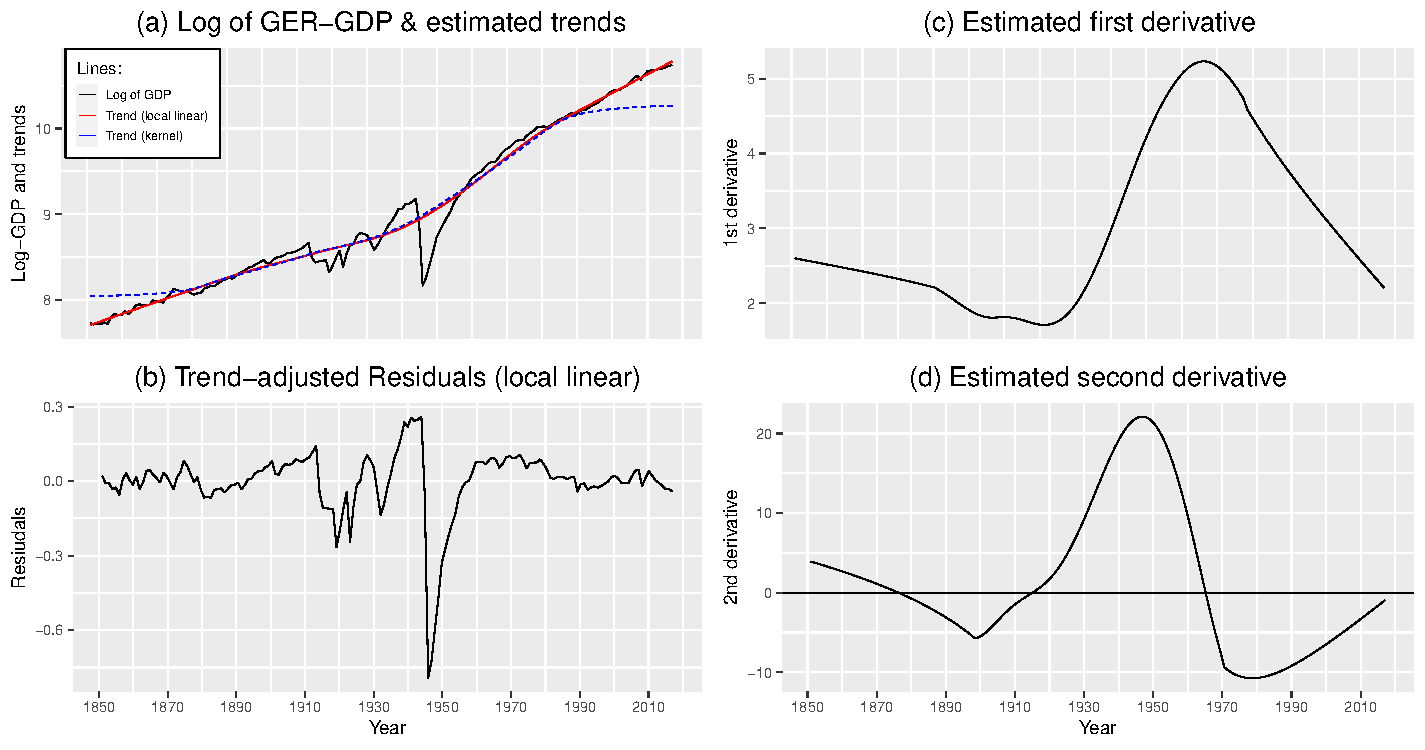
\includegraphics[trim = {0cm 0mm 0mm 0mm}, width = \textwidth]{Abb/GERgdp.pdf}
	\caption{Estimated trend, residuals and the trend`s derivatives for the GER-GDP series}
\end{figure}


\section{Application to high-frequency data}
The autoregressive conditional heteroscedasticity (ARCH) model proposed by \citet{engle1982autoregressive} and its generalisation, the generalized ARCH (GARCH)) model, introduced by \citet{bollerslev1986generalized} , is a well-known volatility process approach for modelling non-constant conditional variances. \citet{feng2004simultaneously} found that return series often simultaneously exhibit conditional heteroskedasticity and a slowly changing scale. Under regular conditions a process with conditional heteroskedasticity is covariance stationary, but a process with change in volatility is at best locally stationary. However, the majority of GARCH extensions are defined assuming a stationary return series. Based on his findings the author proposed the Semi-GARCH model by adding a smooth scale function to the standard GARCH model. Recently, Feng et al. (forthcoming) introduced the Semi-Log-GARCH model which is an extension of the Log-GARCH introduced by \citet{pantula1986modeling}, \citet{geweke1986comment} and \citet{milhoj1987conditional}. Moreover, \citet{feng2020fractionally} and Letmathe et al. (forthcoming) proposed the FI-Log- and Semi-FI-Log-GARCH models, respectively. The FI-Log-GARCH is a special case of the FIAPARCH.

Let $r^*_t$, $t = 1,...,n$ denote a return series with $E(r^*_t) = \mu_{r^*}$. We have
\begin{equation}
	\label{SEMIFIL}
	r_t=\sigma(\tau_t) \sqrt{h_t} \eta_t,
\end{equation}
where $r_t = r_t^* - \mu_{r^*}$ are the centralized returns, $\sigma^2(x_t) >0$ stands for a smooth scale function and $\eta_t$ is defined as in \eqref{MEM}. Let $\xi_t^2=r_t^2 / \sigma^2(\tau_t)=h_t \eta_t^2$ and  $\alpha_{d,i} = \psi(B) - \phi(B)(1-B)^d$, where $\phi(B) = 1 - \sum_{i = 1}^{p^*}\alpha_i B^i - \sum_{j = 1}^{q}\beta_jB^j$ with $p^* = \max(p,q)$ and $\psi(B) = 1 + \sum_{j=1}^{q}\psi_jB^j = 1 - \sum_{j = 1}^{q}\beta_jB^j$. Furthermore, $\alpha_i$ and $\beta_j$ are the ARCH and GARCH coefficients, respectively. $\{\xi_t\}$ is assumed to follow a FI-Log-GARCH process given by 
\begin{equation}
	\label{SEMIFIL*}
	\ln h_t = \alpha_0 + \sum_{i = 1}^{\infty}\alpha_{d,i} \ln \xi_{t-1}^2 + \sum_{j = 1}^{q} \beta_j \ln h_{t-j},	
\end{equation}
where $\alpha_0$ is some constant. \eqref{SEMIFIL} and \eqref{SEMIFIL*} together define a SEMI-FI-Log-GARCH. To ensure that our model is well defined we assume that $\xi_t \neq 0$ a.s. and $\var(\xi_t) = 1$. Let $y_t = \ln r^2_t$, $g(\tau_t) = \ln \sigma^2(\tau_t) + \mu_{l\xi^2}$ and $Z_t = \ln \xi^2_t - \mu_{l\xi^2}$, where $\mu_{l\xi^2} = E(\ln \xi_t^2)$. 
We can see that the log-transformation of the Semi-FI-Log-GARCH defined by \eqref{SEMIFIL} and \eqref{SEMIFIL*}  admits an additive model form $y_t = g(\tau_t) + Z_t$, which is a special case of Model \eqref{SEMIFAR}. Moreover, let $\epsilon_t = \ln \eta^2 - \mu_{l\epsilon^2}$, with $\mu_{l\epsilon^2} = E(\ln \eta^2_t)$ and then we have $Z_t = \ln h_t + \epsilon_t - (\mu_{l\xi^2} - \mu_{l\epsilon^2})$. It was shown by \citet{feng2020fractionally} that $Z_t$ can be represented as a FARIMA($p^*,d,q$) model given by 
\begin{equation}
	(1-B)^d\phi(B)(Z_t) = \psi(B)\epsilon_t,	
\end{equation}
which is in turn a special case of Model \eqref{FARIMA}. We see that the Semi-FI-Log-GARCH is equivalent to a SEMIFARIMA model with the restriction $p \geq q$. Subsequently, well developed SEMIFARIMA algorithms are applicable for estimating $g(\tau_t)$ and $Z_t$. %Then $\hat{h}_t$ and  by  $\hat{h}_t = \hat{C}_\sigma \hat{h}_t^*$, with $\hat{h}_t^* = \exp(\hat{Z}_t)$
$\hat{\sigma}(\tau_t)$ can be obtained by $\hat{\sigma}(\tau_t) = \hat{C}_\sigma \exp [\hat{g}(\tau_t) / 2]$, where $C_\sigma^2 = \var (r_t / \exp[g(\tau_t) / 2])$. $C_\sigma$ can be estimated consistently by the scale-adjusted returns under the assumption that $E(\xi_1^4)<\infty$.

The Semi-FI-Log-GARCH is applied to 


\section{The Semi-FI-Log-ACD model* (nachfragen)}

\section{Concluding remarks}

\printbibliography

\section*{Appendix}





\end{document}
